\chapter{INTERPRETAÇÃO DOS RESULTADOS OBTIDOS}
<<<<<<< HEAD
\label{chap:resultados}
O modelo linear encontrado, considerando a interação entre dois elementos, é disposto a seguir.
=======
O modelo de regressão linear encontrado, considerando a interação entre dois elementos, é disposto a seguir.
>>>>>>> feature/results

\begin{knitrout}
  \definecolor{shadecolor}{rgb}{0.969, 0.969, 0.969}\color{fgcolor}\begin{kframe}
  \begin{verbatim}
  ## 
  ## Call:
  ## lm(formula = tempo ~ (altura + clipe + ad_top + ad_esquerda + 
  ##     ad_direita) + altura * clipe + altura * ad_top + altura * 
  ##     ad_esquerda + altura * ad_direita + clipe * ad_top + clipe * 
  ##     ad_esquerda + clipe * ad_direita + ad_top * ad_esquerda + 
  ##     ad_top * ad_direita + ad_esquerda * ad_direita,
  ##     data = helicoptero)
  ## 
  ## Residuals:
  ##       Min        1Q    Median        3Q       Max 
  ## -0.180625 -0.055312 -0.009375  0.059687  0.120625 
  ## 
  ## Coefficients:
  ##                          Estimate Std. Error t value Pr(>|t|)    
  ## (Intercept)               1.24188    0.07069  17.569 6.99e-12 ***
  ## altura+                   0.42125    0.07903   5.330 6.77e-05 ***
  ## clipe+                   -0.04125    0.07903  -0.522  0.60885    
  ## ad_top+                   0.07875    0.07903   0.996  0.33386    
  ## ad_esquerda+              0.17625    0.07903   2.230  0.04040 *  
  ## ad_direita+               0.19125    0.07903   2.420  0.02779 *  
  ## altura+:clipe+           -0.03250    0.07069  -0.460  0.65186    
  ## altura+:ad_top+           0.09500    0.07069   1.344  0.19771    
  ## altura+:ad_esquerda+     -0.04000    0.07069  -0.566  0.57932    
  ## altura+:ad_direita+      -0.02000    0.07069  -0.283  0.78085    
  ## clipe+:ad_top+           -0.03750    0.07069  -0.531  0.60304    
  ## clipe+:ad_esquerda+       0.06750    0.07069   0.955  0.35382    
  ## clipe+:ad_direita+       -0.14250    0.07069  -2.016  0.06092 .  
  ## ad_top+:ad_esquerda+     -0.13500    0.07069  -1.910  0.07425 .  
  ## ad_top+:ad_direita+      -0.00500    0.07069  -0.071  0.94448    
  ## ad_esquerda+:ad_direita+ -0.21000    0.07069  -2.971  0.00901 ** 
  ## ---
  ## Signif. codes:  0 '***' 0.001 '**' 0.01 '*' 0.05 '.' 0.1 ' ' 1
  ## 
  ## Residual standard error: 0.09996 on 16 degrees of freedom
  ## Multiple R-squared:  0.9161,	Adjusted R-squared:  0.8375 
  ## F-statistic: 11.65 on 15 and 16 DF,  p-value: 6.57e-06
  \end{verbatim}
  \end{kframe}
  \end{knitrout}

Pode-se observar que, para o nosso modelo, as variáveis que possuem relevância estatística, ou seja Pr $<$ 0.05 são: altura (Pr = 6.77e-05), ad\_esquerda (Pr = 0.4040), ad\_direita (Pr = 0.02779) e ad\_esquerda:ad\_direita (Pr = 0.00901). 

Considerando as variáveis que possuem relevância estatística, a equação linear que representa o modelo é descrita da seguinte forma:

\begin{center}
\small  
$
  tempo = média(tempos) + \dfrac{coef(altura)}{2}altura + \dfrac{coef(ad\_esquerda)}{2}ad\_esquerda + \dfrac{coef(ad\_direita)}{2}ad\_direita +  \dfrac{coef(ad\_esquerda:ad\_direita)}{2}ad\_esquerda:ad\_direita
$  
\end{center}
\normalsize
Desta forma, fazendo as devidas substituições, temos que:


  $
     tempo = 1.54 + \dfrac{0.42125}{2}altura + \dfrac{0.17625}{2}ad\_esquerda + \dfrac{0.19125}{2}ad\_direita \\ +  \dfrac{(-0.21)}{2}ad\_esquerda:ad\_direita
  $, logo: 

\begin{equation}
\begin{gathered}  
tempo = 1.54 + 0.210625altura + 0.088125ad\_esquerda + 0.095625ad\_direita - \\
0.105ad\_esquerda:ad\_direita
\label{eq:tempo}
\end{gathered}
\end{equation}



É fácil de verificar na equação \ref{eq:tempo} que as variáveis \textit{altura}, \textit{ad\_direita} e \textit{ad\_esquerda} influenciam positivamente no tempo de queda (possuem coeficientes positivos) enquanto a interação entre as variáveis \textit{ad\_esquerda:ad\_direita} influencia negativamente (possui coeficiente negativo). Desta forma, considerando que nossas variáveis de entrada assumam apenas valores de -1 ou 1, para encontrar o maior valor de tempo de voo devemos atribuir valor positivo às variáveis \textit{altura}, \textit{ad\_direita} e valor negativo à interação \textit{ad\_esquerda:ad\_direita}, o que resulta em:

  $tempo\_max =  1.54 + 0.2106*(1) + 0.0881*(1) + 0.0931*(1) - 0.105*(-1) = 2.04seg$

De forma análoga, para encontrar o menor valor de tempo de voo devemos atribuir valor negativo às variáveis \textit{altura}, \textit{ad\_direita} e \textit{ad\_esquerda} e valor positivo à interação \textit{ad\_esquerda:ad\_direita}, resultando em :

  $tempo\_min =  1.54 + 0.2106*(-1) + 0.0881*(-1) + 0.0931*(-1) - 0.105*(1) = 1.15seg$

Os valores esperados para cada teste de lançamento do helicóptero(\textit{Tempo}), bem como os previstos pelo modelo de regressão linear(\textit{Tempo\_p}) e seus respectivos resíduos podem ser visualizados na Tabela \ref{tab:residuos}.

\begin{table}[H]
  \small
  \center
  \caption{Valores Previstos e Resíduos}
  \begin{tabular}{|c|c|c|}
  \hline
  \textbf{Tempo} & \textbf{Tempo\_p} & \textbf{Resíduo} \\ \hline
  1,27           & 1,241875          & 0,028125         \\ \hline
  1,57           & 1,663125          & -0,093125        \\ \hline
  1,1            & 1,200625          & -0,100625        \\ \hline
  1,7            & 1,589375          & 0,110625         \\ \hline
  1,31           & 1,320625          & -0,010625        \\ \hline
  1,82           & 1,836875          & -0,016875        \\ \hline
  1,3            & 1,241875          & 0,058125         \\ \hline
  1,75           & 1,725625          & 0,024375         \\ \hline
  1,36           & 1,418125          & -0,058125        \\ \hline
  1,92           & 1,799375          & 0,120625         \\ \hline
  1,52           & 1,444375          & 0,075625         \\ \hline
  1,71           & 1,793125          & -0,083125        \\ \hline
  1,4            & 1,361875          & 0,038125         \\ \hline
  1,83           & 1,838125          & -0,008125        \\ \hline
  1,32           & 1,350625          & -0,030625        \\ \hline
  1,74           & 1,794375          & -0,054375        \\ \hline
  1,5            & 1,433125          & 0,066875         \\ \hline
  1,91           & 1,834375          & 0,075625         \\ \hline
  1,23           & 1,249375          & -0,019375        \\ \hline
  1,55           & 1,618125          & -0,068125        \\ \hline
  1,42           & 1,506875          & -0,086875        \\ \hline
  2,04           & 2,003125          & 0,036875         \\ \hline
  1,35           & 1,285625          & 0,064375         \\ \hline
  1,68           & 1,749375          & -0,069375        \\ \hline
  1,44           & 1,399375          & 0,040625         \\ \hline
  1,58           & 1,760625          & -0,180625        \\ \hline
  1,25           & 1,283125          & -0,033125        \\ \hline
  1,73           & 1,611875          & 0,118125         \\ \hline
  1,32           & 1,338125          & -0,018125        \\ \hline
  1,86           & 1,794375          & 0,065625         \\ \hline
  1,17           & 1,184375          & -0,014375        \\ \hline
  1,63           & 1,608125          & 0,021875         \\ \hline
  \end{tabular}
  \label{tab:residuos}
  \end{table}

De posse desses valores, para garantir a veracidade do modelo de regressão linear encontrado deve-se então realizar à análise dos seus resíduos, os quais espera-se possuírem distribuição normal e aleatoriedade em torno da regressão obtida.  A Figura \ref{fig:hist_residuals} exibe o histograma dos resíduos calculados e pode-se observar a distribuição normal dos valores, conforme o esperado.

\begin{figure}[H]
  \caption{Histograma dos resíduos}
  \center
  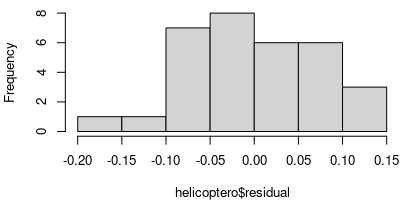
\includegraphics[scale=0.7]{images/hist_residuals.png}
  \legend {Fonte: Autoria própria.}
  \label{fig:hist_residuals}
\end{figure}

Ao usar a função \textbf{plot()} para o nosso modelo, o primeiro gráfico gerado é o \textit{Residuals vs Fitted}, exibido na Figura \ref{fig:fitted}, que dá uma indicação se há padrões não-lineares nos resíduos. Pode-se verificar na figura que o nosso modelo exibe uma regressão linear atráves de um certo número dos pontos.

\begin{figure}[H]
\caption{\textit{Residuals vs Fitted}}
\center 
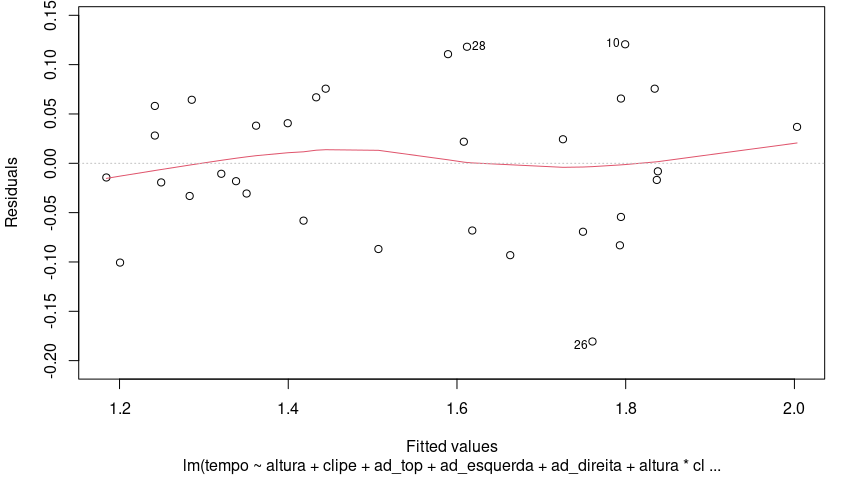
\includegraphics[scale=0.48]{images/fitted.png}
\legend {Fonte: Autoria própria.}
\label{fig:fitted}
\end{figure}

Uma outra forma de verificar a distribuição normal dos resíduos é através da Normal Q-Q. Podemos visualizar na Figura \ref{fig:qq} a Normal Q-Q para o nosso modelo, na qual os resíduos seguem próximos à linha reta em diagonal, sendo uma boa indicação de que encontram-se normalmente distríbuidos.

\begin{figure}[H]
  \caption{Normal Q-Q}
  \center
  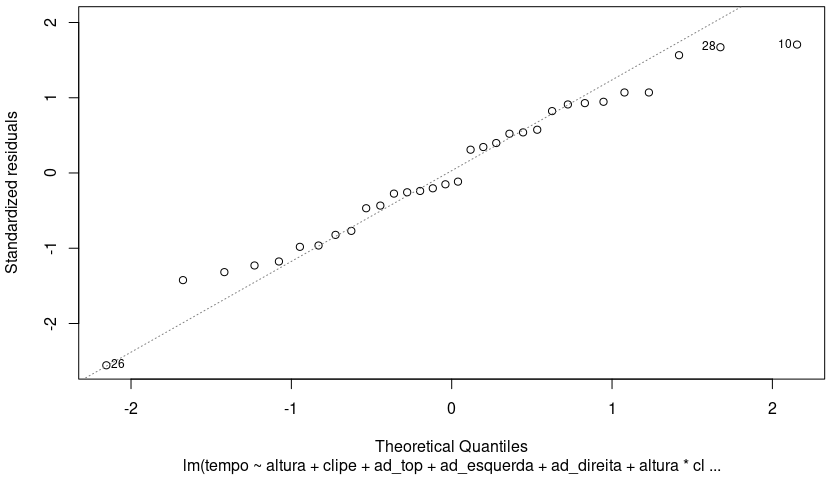
\includegraphics[scale=0.48]{images/qq.png}
  \legend {Fonte: Autoria própria.}
  \label{fig:qq}
\end{figure}

É necessário verificar também se os resíduos possuem homocedasticidade, ou seja possuam variância comum ao longo da regressão. Pode-se observar no gráfico exibido na Figura \ref{fig:scale} que os resíduos apresentam-se aleatoriamente pela linha, sem concentrar-se nem ao topo nem abaixo da mesma, comportamento que se assemelha ao esperado.

\begin{figure}[H]
  \caption{\textit{Scale-Location}}
  \center 
  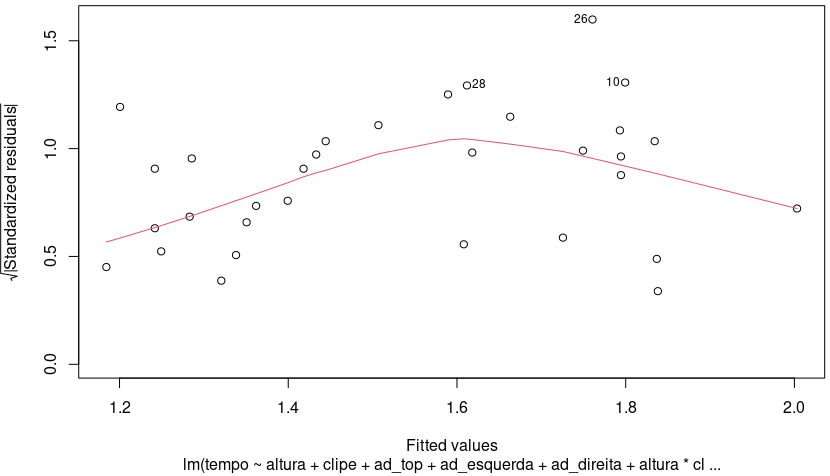
\includegraphics[scale=0.48]{images/scale_location.png}
  \legend {Fonte: Autoria própria.}
  \label{fig:scale}
\end{figure}

A partir da análise realizada dos resíduos é possível então inferir que o modelo de regressão linear encontrado na equação \ref{eq:tempo} é válido para o helicóptero de papel utilizado, com as varíaveis \textit{altura}, \textit{ad\_direita} e \textit{ad\_esquerda} possuindo relevância para a resposta observada na variável de saída (\textit{tempo}).